\documentclass[12pt]{article}
\usepackage{graphicx}
\usepackage{hyperref}
\usepackage{listings}
\usepackage{graphicx}
\usepackage[T1]{fontenc}
\usepackage[polish]{babel}

\graphicspath{ {./images/} }

\lstset{mathescape}

\title{Raport projektu - \textit{Connect Four}}
\author{Mateusz Tkaczyk \\ Jakub Rudnik \\ Piotr Kurosad \\ Filip Łojek}
\date{8 marca 2024}

\begin{document}

\maketitle

\begin{abstract}
    Celem tego projektu było stworzenie modelu uczenia maszynowego zdolnego do skutecznego grania w grę \textit{Connect Four}. Aby osiągnąć ten cel, zaprojektowaliśmy i wdrożyliśmy dwa różne podejścia: regresyjne i klasyfikacyjne. Model regresyjny został zaprojektowany do przewidywania liczbowych wartości wyjściowych, reprezentujących ocenę danej pozycji. Natomiast model klasyfikacyjny miał na celu wytypowanie najlepszego ruchu spośród możliwych opcji, traktując to jako problem klasyfikacji.
\end{abstract}

\clearpage

\tableofcontents

\clearpage

\section{Wprowadzenie do projektu}

\subsection{Narzędzie i technologię}

W ramach naszego projektu korzystaliśmy z szeregu technologii i narzędzi, które umożliwiły efektywne stworzenie oraz wdrożenie modelu uczenia maszynowego do gry \textit{Connect Four}, jak również interaktywnego interfejsu użytkownika.

Cały projekt został napisany w języku \href{https://www.python.org/}{Python3}, korzystaliśmy z najnowszej na tamtą chwilę wersji \href{https://www.python.org/downloads/release/python-3119/}{3.11.9}. Do stworzenia modelu wykorzystaliśmy bibliotekę \href{https://www.tensorflow.org/}{TensorFlow} w wersji 2.16.1. Interfejs użytkownika został zaprogramowany dzięki użyciu biblioteki \href{https://www.pygame.org}{pygame} w wersji 2.5.2. Dodatkowo korzystaliśmy z dodatkowych narzędzi do pomniejszych zadań takich jak rozdzielenie zbiorów na treningowy i testowy za pomocą \href{https://scikit-learn.org/}{sklearn}, wczytanie danych dzięki \href{https://pandas.pydata.org/}{pandas}. Kluczową biblioteką, która była odpowiedzialna za operację na danych (oraz jest wewnętrznie wykorzystywana przez TensorFlow) jest \href{https://numpy.org/}{numpy}.

\subsection{Opis modeli}
Zadaniem algorytmu jest gra w klasyczną wersję \textit{Connect Four}. Użytkownik za pomocą interfejsu graficznego, będzie mógł grać przeciwko wybranemu algorytmowi. Do wyboru będą dwa modele:
\begin{itemize}
    \item klasyfikacyjny, w którym odpowiedzią modelu będzie ruch (dokładnie jego indeks od 0 do 6),
    \item regresywny, w którym odpowiedzią modelu będzie ewaluacja danej pozycji (dodatnie wartości świadczą o wygrywającej pozycji aktualnego gracza, 0 o remisie, a ujemne wartości o przegrywającej pozycji).
\end{itemize}

\noindent Danymi wejściowymi będzie plansza gry oraz informacja o tym, kto wykonuje następny ruch. Możliwe, że do modeli zostaną dostarczone dodatkowe informacje w zależności od potrzeb.


Dane treningowe oraz ewaluacyjne zostaną wygenerowane przez jeden z dostępnych silników do gry w \textit{Connect Four}.

\subsection{Zbieranie danych}
Dane zostały zebrane za pomocą optymalnego bota do \textit{Connect Four}. Ma on przeliczoną całą grę i mamy pewność, że dla każdej pozycji zwróci on nam dokładną ewaluację każdego ruchu. Ewaluuje on pozycje w następujący sposób (zakładając optymalny przebieg rozgrywki po każdym ruchu):

\begin{itemize}
    \item Jeśli po danym ruchu jesteśmy w stanie wygrać grę, to wynik tej ewaluacji jest dodatni.
    \item Jeśli po danym ruchu jesteśmy w stanie tylko przegrać, wynik ewaluacji jest ujemny.
    \item Jeśli dany ruch prowadzi do remisu, wynik ewaluacji to 0.
    \item Im wyższy
          wynik dodatni, tym szybciej po danym ruchu możemy wygrać, im bardziej ujemny wynik tym szybciej przegrywamy.
\end{itemize}

Dane zbieramy w następującym formacie:

\begin{lstlisting}
    $opis\_pozycji$, $ewaluacja_1$, $ewaluacja_2$, ..., $ewaluacja_7$
\end{lstlisting}


gdzie $opis\_pozycji$ jest wypisanymi jeden po drugim liczbami, oznaczającymi kolejne ruchy (indeksy kolumn, do których wrzucane były żetony) prowadzące do obecnej pozycji. $ewaluacja_i$ oznacza natomiast ewaluację ruchu do $i$-tej kolumny przy obecnej pozycji. Zdecydowaliśmy się dodatkowo na zebranie danych następującymi sposobami:

\begin{itemize}
    \item patrząc tylko na możliwe optymalne ruchy, budujemy drzewo optymalnych strategii,
    \item patrząc na wszystkie możliwe rozgrywki do danej głębokości, wygenerowaliśmy wszystkie rozgrywki do 8 ruchów od początku gry,
    \item generując zupełnie losowe rozgrywki,
    \item generując losowe rozgrywki, ale im lepszy ruch, tym większe prawdopodobieństwo mamy na jego wybranie.
\end{itemize}

Przy każdym z tych sposobów, każda wygenerowana pozycja ma przypisaną ewaluację każdego możliwego ruchu. Dzięki takiemu generowaniu danych, mamy nadzieję, że algorytm będzie w stanie poradzić sobie z graczem grającym dobre ruchy, ale jednocześnie powinien umieć wykorzystać błędy swojego przeciwnika.

\section{Opisy modeli}

\subsection{Model regresywny z planszą jako daną wejściową}

\subsubsection{Dane wejściowe}

Początkowa próba stworzenia modelu regresywnego opierała się na jednej danej wejściowej. Była to macierz o rozmiarach (6, 7, 2) składająca się z wartości logicznych. Reprezentowała ona jednoznacznie planszę do gry w \textit{Conenct Four}. Wymiary (6, 7) odpowiadają wymiary planszy, a dodatkowy wymiar o wielkości 2, skorelowany jest z danym graczem. Jeżeli krążek pierwszego gracza znajduje się na planszy to w macierzy będzie symbolizowany jako wartość prawdziwa. Analogicznie dla drugiego gracza pamiętając, że żetony pierwszego gracza znajdują się w zerowej warstwie, a drugiego w kolejnej.

\begin{figure}[!ht]
    \centering
    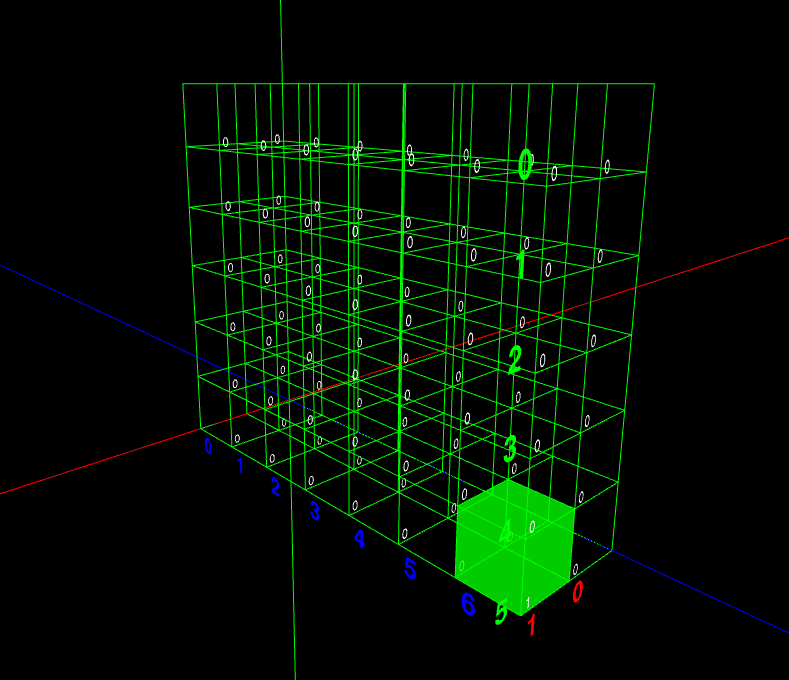
\includegraphics[scale=0.40]{board.png}
    \caption{Wizualna reprezentacja macierzy planszy, gdzie pierwszy gracz wykonał jedyny ruch na 6 kolumnie.}
\end{figure}

W trakcie pracy nad modelem zdaliśmy sobie sprawę, że istotną informacją jaką należałoby dodać jest zmienna mówiąca, który gracz wykona najbliższy ruch. Dla człowieka (lub innego rodzaju algorytmu) taka informacja może okazać się zbędna, ponieważ przy poprawnym tworzeniu planszy parzystość żetonów definiuje osobę, która wykonuje następny ruch. Jeżeli liczba jest nieparzysta pierwszy gracz musiał wykonać więcej ruchów, zatem następny powinien ruszyć się drugi gracz. W przeciwnym wypadku rusza się gracz pierwszy.

Zatem końcowo model jako dane wejściowe posiadał macierz o rozmiarach (6, 7, 2) jednoznacznie reprezentującą planszę oraz zmienną określającą gracza, który wykonuje ruch.

\subsubsection{Wielkość danych treningowych i testowych}

Podczas tworzenia modeli, do naszej dyspozycji było około 22 milionów plansz wraz z ich ewaluacjami. Jednak trenowanie na wszystkich dostępnych danych szybko okazał się nieefektywnym sposobem tworzenia modeli. Wielkość modelu, zmienną po której ocenialiśmy jego jakość i inne jego parametry zmienialiśmy w sposób dynamiczny analizując jakość uzyskanego algorytmu. Dzięki trenowaniu przy użyciu mniejszej ilości danych (około 100 tysięcy) byliśmy w stanie dostosowywać i zmieniać paramenty modelu w znacznie szybszy sposób.

Do testowania modelu podeszliśmy w sposób bardziej kompleksowy. Zależało nam, aby wynik ewaluacji jakości modelu w jak najlepszy sposób odpowiadał jego rzeczywistej sile gry. Dlatego przy testowaniu każdego modelu używaliśmy wszystkich danych jakie mieliśmy do dyspozycji. Nawet jeżeli dany model był trenowany na mniejszej ilości danych, jego końcowa ewaluacja odbywała się na całym zbiorze.

\subsubsection{Rozmiar modelu w kontekście siły gry}

Pierwsze stworzone przez nas modele, miały dość mały rozmiar (około 40 tysięcy parametrów). W pewnym momencie, kolejne iteracje nie poprawiały jakości modelu. Kiedy pojawiał się taki problem, analizowaliśmy czy model nie potrzebuje innych danych wejściowych lub zmiany zbioru danych treningowo-testowych. Następnie zwiększaliśmy liczbę jego parametrów. Taka zmiana poprawiała ewaluację danego modelu, nie tylko statystycznie, lecz również rosła realna siła gry algorytmu. Ostateczny model posiada około 84 milionów parametrów. Możliwym jest, że taka liczba parametrów przerasta liczbę stopni swobody gry w \textit{Connect Four}, ciężko jednak mówić o stopniach swobody, kiedy analizujemy teorie gier. Trudno jest stwierdzić, kiedy rozmiar modelu jest zbyt duży i zwiększanie go, nie przynosi realnych korzyści. Wówczas algorytm dopasowuje się do danych jakimi go posiłkujemy, a nie do realnych zasad gry.

\subsubsection{Realna siła gry}

W trakcie rozwoju modelu opartego o planszę, jego jakość znacznie się zwiększała. Każda kolejna iteracja, czy to zmieniająca dane wejściowe, treningowe czy liczbę parametrów, poprawiała siłę analizy naszego algorytmu. Niestety te podejście spotkało się z pewnymi twardymi ograniczeniami, które okazały się dla nas przeszkodą w dalszym rozwijaniu tego podejścia. Nie byliśmy w stanie dalej polepszać jakości algorytmu mimo zastosowania większej ilości danych, parametrów lub zmiany wewnętrznych ustawień (np. optymalizator, zmienna po której oceniamy jakość itd.). W końcowej wersji modelu, nie udało się nam uzyskać satysfakcjonującej siły gry. Algorytm potrafi wykonywać bardzo dobre ruchy, ale nie rozumie podstawowych zasad gry jak obronę kiedy przeciwnik ma 3 żetony w linii. Dochodzi do sytuacji, kiedy nasz model w momencie przegranej w jednym ruchu nie broni się, tylko wybiera inną kolumnę, skutkującą natychmiastową przegraną. Nie tylko ma on trudności z człowiekiem, lecz również zbyt duży opór stanowi dla niego algorytm grający losowo. Zatem te podejście okazało się niepoprawne. Możliwe, że gdybyśmy zastosowali więcej danych wejściowych (np. mówiące o tym, czy przeciwnik ma wygraną w następnym ruchu), nasz algorytm uodpornił by się na ten problem. Postanowiliśmy jednak spróbować rozwinąć nasze inne pomysły, które podchodzą do problemu w całkowicie inny sposób (np. bez podania planszy jako danej wejściowej).

\clearpage

\subsection{Model regresywny z planszą oraz liniami jako danymi wejściowymi}

\subsubsection{Koncepcja linii}
Głównym celem w grze jest połączenie czterech krążków w linię, dlatego dobrze gdybyśmy przekazywali w danych wejściowych do modelu informacje związane z tą koncepcją. Na planszy można stworzyć 69 różnych linii o czterech polach. Zamysłem jest, aby policzyć ile dany gracz ma możliwych linii, na których w przyszłości mógłby ustawić zwycięską linię czterech krążków. Dla każdego z dwóch graczy tablica $[a_1, a_2, a_3, a_4]$ będzie zliczała ilość takich możliwych linii, gdzie pole $a_n$ określa, ile jest linii, w których znajduje się już $n$ krążków zawodnika. Z oczywistych względów w pozostałych miejscach linii znajduje się $4 - n$ pustych pól (nie może znaleźć się tu żaden krążek przeciwnika, ponieważ wtedy nie dałoby się stworzyć tu zwycięskiej linii czterech krążków).
\\ \\
Przykładowo dla takiej pozycji:
\begin{figure}[!ht]
    \centering
    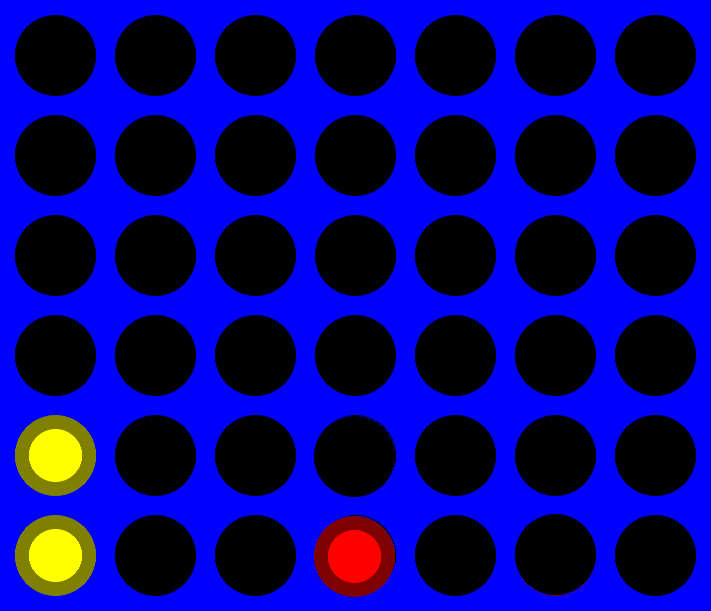
\includegraphics[scale=0.40]{example.png}
    \caption{Przykładowa pozycja na planszy po 3 ruchach.}
\end{figure}

\noindent Dla gracza z żółtymi krążkami tablica linii będzie wynosiła $[4, 1, 0, 0]$, ponieważ posiada jedną potencjalną linię z dwoma krążkami, a reszta to linie z jednym krążkiem. Z kolei dla gracza o czerwonych krążkach tablica wynosi $[6, 0, 0, 0]$. Należy pamiętać, że możliwe są aż trzy potencjalne linie w poziomie z tym krążkiem.

\subsubsection{Dane wejściowe}

Dane wejściowe modelu to plansza, zapisana w takiej samej postaci jak wcześniej opisana. Dodatkowo przekazywane są dwie tablice o rozmiarze (4, 1) - tablica linii dla gracza pierwszego oraz tablica linii dla gracza drugiego.

\subsubsection{Wielkość danych treningowych i testowych}

Niestety przy takich danych wejściowych nie można było przekazywać do modelu jedynie pozycji, ale należało przekształcić te dane zliczając ilość linii. Koszty takie operacji są duże, ponieważ każdy z krążków należy do wielu potencjalnych linii. Przez to zmniejszyliśmy ilość dostarczanych danych podczas trenowania.

\subsubsection{Realna siła gry}
Niestety podejście to również nie przyniosło spodziewanego rezultatu. Model mimo dodatkowej informacji zawartej tablicach odnośnie linii nie wykazał znacznej poprawy w porównaniu do modelu bez linii. Model zdaje się wykonywać losowe ruchy. Nie broni się także blokując linię przeciwnika,  w której ma już on trzy krążki swojego koloru.

\subsection{Model regresywny tylko z liniami jako dane wejściowe}

\subsubsection{Dane wejściowe}

Być może modelowi, który jako argumenty wejściowe miał podawaną zarówno planszę jak i linie, ciężko było zinterpretować dodatkowe parametry w postaci linii, skoro miał już przekazywaną całą pozycję. W tym podejściu zrezygnowaliśmy z przekazywania pozycji, wybierając na dane wejściowe jedynie tablice linii dla obydwu graczy. Model nie miał przez to pełnej informacji jaka była pozycja na planszy, jednak linie przekazywały dużo informacji w kontekście zasad gry. Model na podstawie trenowania powinien wywnioskować, że im więcej własnych potencjalnych linii w pozycji, tym lepiej powinien ją oceniać.

\subsubsection{Wielkość danych treningowych i testowych}

Wielkości danych, ale także sposób trenowania były analogiczne jak w przypadku poprzedniego modelu, z danymi wejściowymi pozycji i tablicami linii.

\subsubsection{Realna siła gry}
To podejście okazało się również niewystarczające. Model zachowywał się podobnie do poprzedniego. Z perspektywy człowieka wykonywał on losowe ruchy. Nie bronił się także przed przegraną. To zapoczątkowało wątpliwości, czy tablice linii są odpowiednim rodzajem danych przekazywanych do modelu. Mówią one jedynie, ile jest linii, nie biorąc pod uwagę ich jakości. Przykładowo w danej pozycji może nastąpić takie ustawienie, że gdy przeciwnik zablokuje nam jedną z linii, to otworzy nam to możliwość na dostawienie własnego krążka do kolejnej linii - być może zwycięskiej. Ze względu na takie wątpliwość powstał kolejny model, który nie był już przeznaczony do gry, ale jako zbadanie czy podejście tablicy linii ma jakikolwiek sens.

\subsection{Model regresywny tylko z liniami - eksperyment}

Jak opisano w poprzednim akapicie, zastosowanie tablic linii jako danych wejściowych wzbudziło wątpliwości. Dlatego został stworzony prosty model, który przyjmuje dwie tablice linii, dla każdego z graczy. Warstwa ta jest bezpośrednio połączona z wyjściem, dlatego model posiada tylko 9 parametrów - 8 wag połączeń oraz bias.

\begin{figure}[!ht]
    \centering
    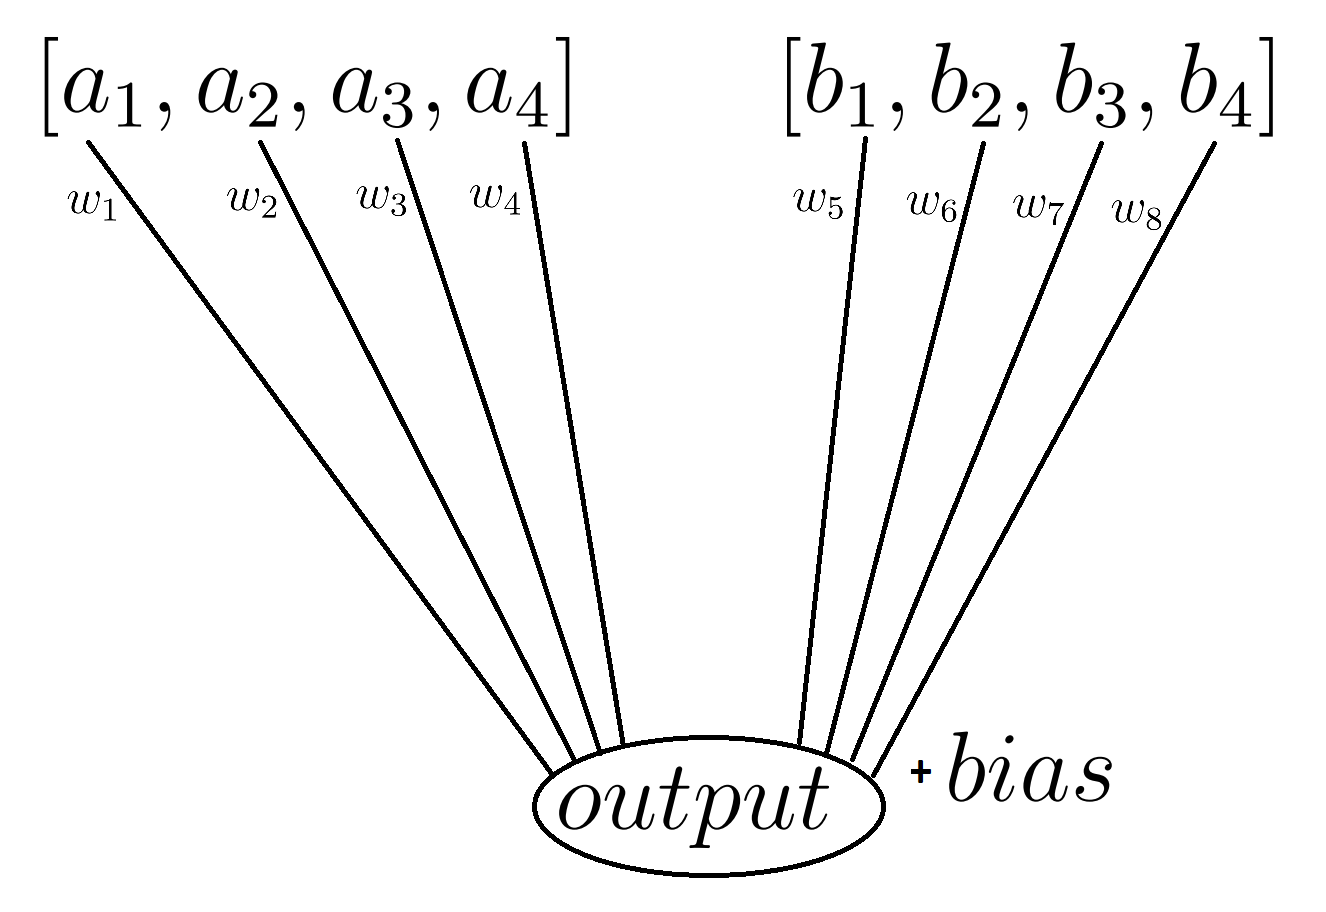
\includegraphics[scale=0.40]{parameters.png}
    \caption{Wizualizacja parametrów modelu eksperymentalnego - 8 wag połączeń oraz bias.}
\end{figure}

\noindent Jeżeli przeanalizujemy zasady gry, powinniśmy mieć pewne oczekiwania w stosunku do wartości tych parametrów:

\begin{itemize}
    \item Każdy z graczy wygrywa poprzez te same zasady, dlatego wartość \textit{bias}-u nie powinna faworyzować żadnego z graczy. Dodatkowo wartości linii o danej ilości własnych krążków powinny być takie same dla obu graczy.
    \item Tablica z wartościami $a_n$ odpowiada za linie gracza pierwszego (żółte krążki), który ma za zadanie maksymalizować wynik. Analogicznie tablica druga z wartościami $b_n$ odpowiada za gracza drugiego (czerwone krążki), który minimalizuje wynik,
    \item Linia, w której gracz posiada więcej własnych krążków powinna być lepsza od tej, w której jest ich mniej. Jest to dosyć oczywista zasada, ponieważ jesteśmy wtedy bliżej od zwycięstwa.
\end{itemize}

\noindent Oznacza to, że wartości parametrów powinny mieć następujące własności:

\begin{itemize}
    \item \textit{bias} = 0,
    \item $|a_n| = |b_n|$
    \item $a_n > 0$, $b_n < 0$,
    \item $|a_4| > |a_3| > |a_2| > |a_1|$, $|b_4| > |b_3| > |b_2| > |b_1|$,
\end{itemize}

\noindent Niestety po treningu modelu wartości jego parametrów były dalekie od oczekiwanych, co może sugerować, że ilość potencjalnych linii do zwycięstwa nie jest jednoznacznym wyznacznikiem oceny, jak dobra jest dana pozycja.

\subsection{Model klasyfikacyjny podstawowy}

\subsubsection{Dane wejściowe}

W podstawowej wersji modelu klasyfikacyjnego postanowiliśmy jako daną wejściową podać tak samo jak w modelu 2.1 planszę, zapisaną w postaci trójwymiarowej macierzy o rozmiarze (6,7,2), której szczegóły objaśnione są w sekcji 2.1.1. Oprócz reprezentacji planszy podajemy zmienną typu boolowski określającą kto wykonuje teraz ruch.

\subsubsection{Wielkość danych treningowych i testowych}

Dogenerowaliśmy w międzyczasie około 2 milionów danych testowych, co z wcześniejszymi danymi daje niespełna 25 milionów plansz i ich ewaluacje. Trenowanie odbywało się na losowo wybranych rekordach z tychże danych, dzięki czemu czas trenowania był dużo krótszy a jakość treningów nie spadała znacząco w stosunku do trenowania na pełnych zestawach danych. Mimo wszystko do samego testowania postanowiliśmy użyć wszystkich danych jakie mieliśmy aby otrzymane wyniki testów były jak najbardziej miarodajne.

\subsubsection{Rozmiar modelu w kontekście siły gry}

Początkowo model był małych rozmiarów, lecz w miarę eksperymentowania z dodatkowymi powłokami, ze zwiększaniem ilości neuronów w kolejnych powłokach rozmiar znacznie się zwiększył. Końcowo model zajmuje około 230MB co przekłada się na trochę powyżej 60 milionów parametrów. Przy próbie dalszego zwiększania różnych parametrów modelu nie odnotowaliśmy widocznej poprawy dlatego uznaliśmy obecny model za końcowy.

\subsubsection{Realna siła gry}

Model został poddany treningowi tak długo jak długo rosła dokładność jego odpowiedzi. Dokładność tą badaliśmy za pomocą funkcji bibliotecznej "mean squared error", która liczy średnią kwadratów błędów między odpowiedzią bota, a wynikiem spodziewanym. W pewnym momencie dalsze iteracje nie powodowały poprawy dokładności, a czasem nawet ta dokładność zaczęła maleć więc skończyliśmy trenowanie. Model ten okazał się najlepiej działającym spośród wszystkich stworzonych przez nas modeli. Początkowe ruchy wykonuje on książkowo - dokładnie tak jak to było podane w zbiorze treningowym. W dalszym toku rozgrywki gra całkiem dobrze, zdecydowanie możemy stwierdzić że potrafiłby ograć każdy z pozostałych modeli. Jednak ma ten sam problem co inne modele, nie jest w stanie wykryć tego, że przeciwnik ma już na planszy 3 dyski i często oddaje w ten sposób wygraną przeciwnikowi. Aby tą słabość zniwelować stworzyliśmy model z sekcji 2.4.

\subsection{Model klasyfikacyjny wersja 0-1}

\subsubsection{Dane wejściowe}

Jest to kolejny model klasyfikacyjny, który tak samo jak model 2.2 przyjmuje jako parametry wejściowe macierz o rozmiarze (6,7,2) reprezentującą planszę oraz zmienną wskazującą gracza, który obecnie się rusza. Różnica w porównaniu do poprzedniego modelu polega na formacie danych treningowych. Zamiast podawać dla każdego ruchu ewaluację mającą postać różnych liczb całkowitych zawęziliśmy się do zbioru {0,1}. Oznacza to, że jeśli dany ruch jest najlepszym ruchem w danej sytuacji to jego ewaluacja wynosi 1, w przeciwnym przypadku jego ewaluacja to 0. Należy pamiętać, że najlepszych ruchów może być kilka zatem nie wyklucza to występowania kilku jedynek w tej ewaluacji.

\subsubsection{Wielkość danych treningowych i testowych}

Podczas tworzenia i trenowania tego modelu nie mieliśmy wygenerowanych najnowszych 2 milionów rekordów danych. Trenowanie to zatem odbywało się na pierwszych około 22 milionach danych. Postanowiliśmy sprawdzić, czy zamiast wybierać losowe dane z naszego dużego zbioru, przetrenowanie modelu na całym zestawie danych polepszy końcowe wyniki. Wobec tego zarówno trenowanie, jak i testowanie tego modelu korzystało z całego zbioru 22 milionów rekordów.

\subsubsection{Rozmiar modelu w kontekście siły gry}

Model ten jest wyjątkowo małych rozmiarów, ma niespełna 800 tysięcy parametrów. Tak mały rozmiar spowodowany jest bardzo wczesnym zastojem w zwiększaniu się dokładności w miarę zwiększania ilości parametrów modelu. Wyjątkowo w tym modelu zamiast funkcji "mean squared error" zastosowaliśmy funkcję "binary crossentropy" co wynika z zero-jedynkowości ewaluacji danych treningowych.

\subsubsection{Realna siła gry}

Mimo tego, że trenowaliśmy ten model na całym zbiorze danych treningowych, co jest równoważne z tym że każda iteracja trenowania trwała dłużej niż zwykle to postanowiliśmy konsekwentnie trenować model tak długo, jak długo wartości określające dokładność odpowiedzi będą maleć nawet wtedy gdy już były to bardzo drobne różnice. Ostatecznie model gra nieco ponadprzeciętnie ale popełnia podstawowe błędy. Na pierwsze ruchy nie wybiera środkowej kolumny co jest już poważnym błędem, poza tym nie jest w stanie wykryć tego, że przeciwnik ma już ułożone 3 dyski w rzędzie ale jak już pisaliśmy jest to problem, z którym borykają się wszystkie dotychczas stworzone modele. Uważamy, że działa on lepiej niż gracz wybierający kolumnę losowo, lecz pokonanie tego modelu nie jest dużym wyzwaniem dla człowieka myślącego.

\subsection{Model klasyfikacyjny z dodatkową tablicą czwórek}

\subsubsection{Dane wejściowe}

Tak jak wszystkie poprzednie modele jako dane wejściowe przyjmowane są: macierz o rozmiarze (6,7,2) reprezentująca planszę oraz zmienna mówiąca do kogo należy następny ruch. W końcu aby zapobiec łatwemu podkładaniu zwycięstw przeciwnikowi, postanowiliśmy w ostatnim modelu klasyfikacyjnym jako dodatkowy parametr wejściowy dać tablicę, która będzie wskazywać ile każdy z graczy ma ułożonych dysków w danej czwórce. Dokładniej, plansza o wymiarach (6,7) zawiera w sobie 69 możliwych czwórek jakie można ułożyć - jest to suma wszystkich czwórek poziomych, pionowych i skośnych. Tablica czwórek ma zatem 69 elementów, każdy odpowiada jednej wygrywającej czwórce jaką można ułożyć na planszy. Tablica przyjmuje wartości całkowite od -3 do 3. Gdzie 0 występuje w przypadku gdy każdy z graczy ma co najmniej jeden dysk ułożony w danej czwórce(tam już nikt nie wygra) lub w przypadku gdy czwórka jest pusta. Wartości -3,-2,-1 oznaczają kolejno trzy, dwa, jeden dysk ułożony w danej czwórce przez przeciwnika, podczas gdy pozostałe komórki w czwórce są puste. Wartości 3,2,1 analogicznie tylko oznaczają przewagę grającego.

\subsubsection{Wielkość danych treningowych i testowych}

Ponownie chcąc otrzymać możliwie jak najbardziej dokładne wyniki postanowiliśmy trenować ten model na podstawie całego zbioru danych testowych. Mieliśmy już wtedy dostęp do nowo wygenerowanych danych, co daje w sumie około 24 milionów rekordów. Testowanie również odbywało się przy użyciu całego zbioru danych.

\subsubsection{Rozmiar modelu w kontekście siły gry}

Stworzenie modelu wymagało przetworzenia dodatkowej tabeli wejściowej, stąd od razu rozmiar modelu był spory - nieco ponad milion parametrów. Sukcesywnie dodawaliśmy kolejne warstwy do modelu, które zwiększały dokładność jego odpowiedzi. W chwili gdy dodawanie kolejnych parametrów do modelu nie dawało lepszych wyników, zaprzestaliśmy dalszego zwiększania modelu. Otrzymaliśmy model mający prawie 10 milionów parametrów, co zważywszy na dodatkową tabelę wejściową może nie wydawać się dużym rozmiarem.

\subsubsection{Realna siła gry}

W przypadku tego modelu upłynęła wyjątkowo duża ilość iteracji trenowania zanim przestał on zmniejszać wartości funkcji testującej - "mean squared error". Niestety nie uzyskaliśmy lepszych wyników niż w modelu klasycznym podstawowym, który różni się tylko tym, że nie podajemy na wejściu tablicy czwórek. Być może wystąpiło zjawisko przeuczenia (overfitting), czyli sytuacja, w której model z dużą liczbą parametrów zbyt dokładnie zapamiętuje szczegóły treningowe. Model wtedy działa dobrze na danych treningowych, ale jego wydajność spada na danych testowych lub produkcyjnych, ponieważ nauczy się specyficznych wzorców w danych treningowych zamiast generalnych zależności. Innym powodem niskiej efektywności modelu może być niewłaściwe zaprojektowanie sieci neuronowej, przez którą przechodzą dane wejściowe. Bot potrafi robić dobre ruchy, jednak daleko tutaj od jakiejś reguły, czasami sprawia wrażenie jakby grał losowo.

\end{document}

